\documentclass[../../e3_tp3_main.tex]{subfiles}

\begin{document}

%capítulo
\chapter{Ejercicio 1}

The inputs of the system are $I$ and $S$, and the outputs are $P_1$ and $P_2$. If $P_1=1$ pump 1 is turned on, whereas if $P_1=0$ pump 1 is turned off. The same relation exists between $B_2$ and pump 2. Both FSMs created contemplate the case where the inputs change from $IS=00$ to $IS=11$ and viceversa. If these changes were considered impossible, both implementatios would have two states less. The choice between these two options is determined by the relation between the clock cycle and the rate at which the water level changes: if the clock is much faster, it is guaranteed that there will be no jumps from $IS=00$ to $IS=11$ or viceversa, it would be more conevnient to implement FSM's with less states.

\section{Moore-type FSM implementation}
\subsection{FSM flow-chart}
\begin{figure}[H]
\begin{equation}
	\tikzfig{moore_machine}
\end{equation}
\caption{Flow diagram for the Moore-type FSM implementation. Self loops were ommited for simplicity; they can be found in table \ref{tab:ej1_moore_states}}
\end{figure}

\subsection{State descriptions}
\begin{table}[H]	%moore state descriptions
	\centering
	\begin{tabular}{|c|c|c|c|c|}
	\hline	
	$y_0, y_1, y_2$ & Name & Initials & Description & $P_1$ $P_2$\\	
	\hline 
	000 & Single pump: 1 &SP1& Only pump 1 is on & 10\\ 
	\hline 
	001 & Full, next single pump: 2 &FNSP2 & Pump 1 \& 2 off. Next pump turned on alone: pump 2& 00\\ 
	\hline	
	011 & Empty, next single pump: 2 &ENSP2 & Pump 1 \& 2 on. Next pump turned on alone: pump 2 & 11\\ 
	\hline 
	111 & Single pump: 2 & SP2 & Only pump 2 is on & 01\\ 
	\hline 
	110 & Full, next single pump: 1 &FNSP1& Pump 1 \& 2 off. Next pump turned on alone: pump 1 & 00\\ 
	\hline	
	100 & Empty, next single pump: 1 &ENSP1& Pump 1 \& 2 on. Next pump turned on alone: pump 1 & 11\\ 
	\hline 
	\end{tabular} 
	\caption{Possible states for the Mealy-type FSM implementation.}
	\label{tab:ej1_moore_states}
\end{table}

\subsection{State transition table}
\begin{table}[H]	%moore state transition table
	\centering
		\begin{tabular}{|c|c|c|c|c|}
		\hline 
		state\textbackslash I S & 00 & 01 & 11 & 10 \\ 
		\hline 
		SP1 & ENSP2 & ENSP1 & FNSP2 & SP1 \\ 
		\hline 
		FNSP2 & ENSP2 & ENSP1 & FNSP2 & SP2 \\ 
		\hline 
		ENSP2 & ENSP2 & ENSP1 & FNSP2 & SP2 \\ 
		\hline 
		SP2 & ENSP1 & ENSP1 & FNSP1 & SP2 \\ 
		\hline 
		FNSP1 & ENSP1 & ENSP1 & FNSP1 & SP1 \\ 
		\hline 
		ENSP1 & ENSP1 & ENSP1 & FNSP1 & SP1 \\ 
		\hline 
		\end{tabular} 
	\caption[States transitions and outputs for the Mealy-type FSM implementation]{States transitions and outputs for the Mealy-type FSM implementation.}
	\label{tab:ej1_moore_transitions}
\end{table}

\subsection{Outputs and next states Karnaugh maps}
\begin{figure}[H]
	\centering
	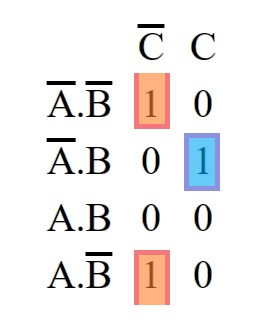
\includegraphics[scale=0.8]{figures/e3_tp3_ej1_moore_b1_kmap.jpg}
	\caption{$P_1$ Karnaugh map}
\end{figure}

\begin{figure}[H]
	\centering
	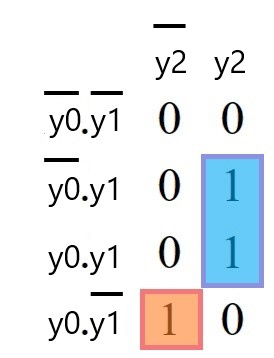
\includegraphics[scale=0.8]{figures/e3_tp3_ej1_moore_b2_kmap.jpg}
	\caption{$P_2$ Karnaugh map}
\end{figure}

\begin{figure}[H]
	\centering
	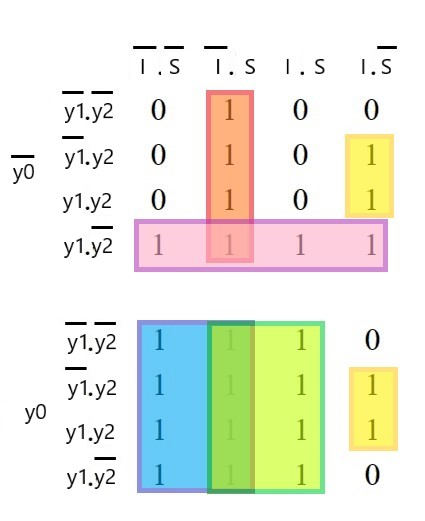
\includegraphics[scale=1]{figures/e3_tp3_ej1_moore_y0_kmap.jpg}
	\caption{$y_0$ Karnaugh map}
\end{figure}

\begin{figure}[H]
	\centering
	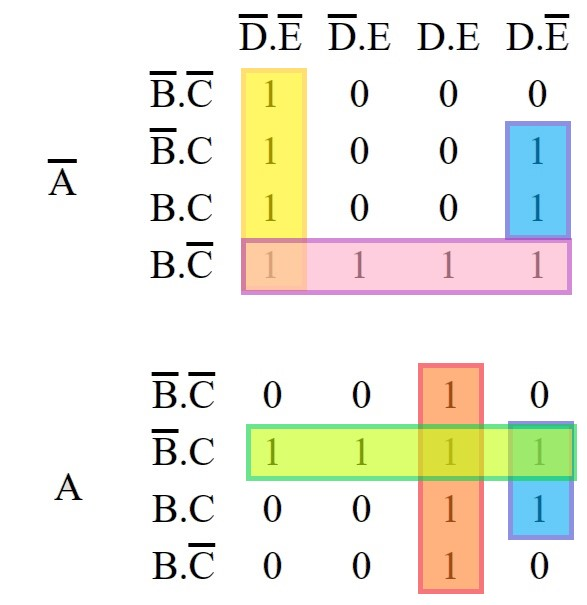
\includegraphics[scale=0.8]{figures/e3_tp3_ej1_moore_y1_kmap.jpg}
	\caption{$y_1$ Karnaugh map}
\end{figure}

\begin{figure}[H]
	\centering
	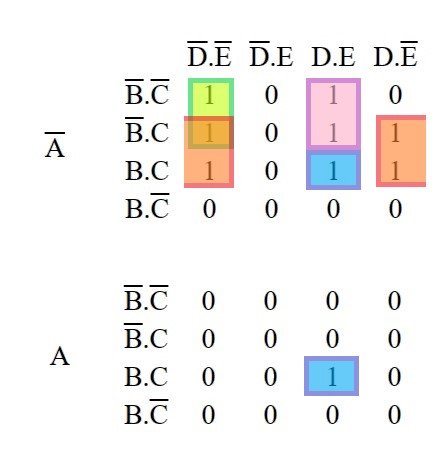
\includegraphics[scale=1]{figures/e3_tp3_ej1_moore_y2_kmap.jpg}
	\caption{$y_2$ Karnaugh map}
\end{figure}


\subsection{Outputs and next states schematics}
%schematics as sum-of-products
\begin{figure}[H]
	\centering
	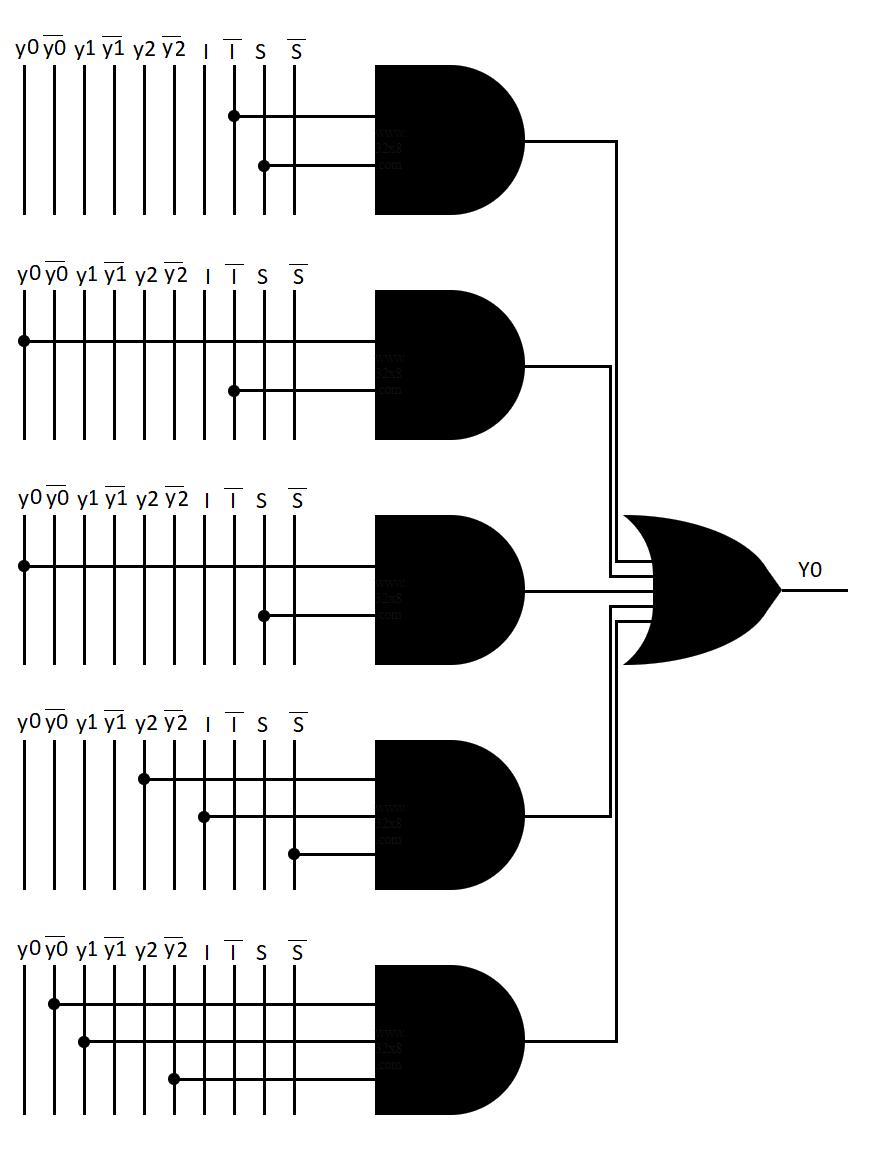
\includegraphics{figures/moore_Y0_schem.PNG}
	\caption{$Y_0$ schematic as a sum-of-products}
	\label{fig:ej1_moore_Y0_schem}
\end{figure}
\begin{figure}[H]
	\centering
	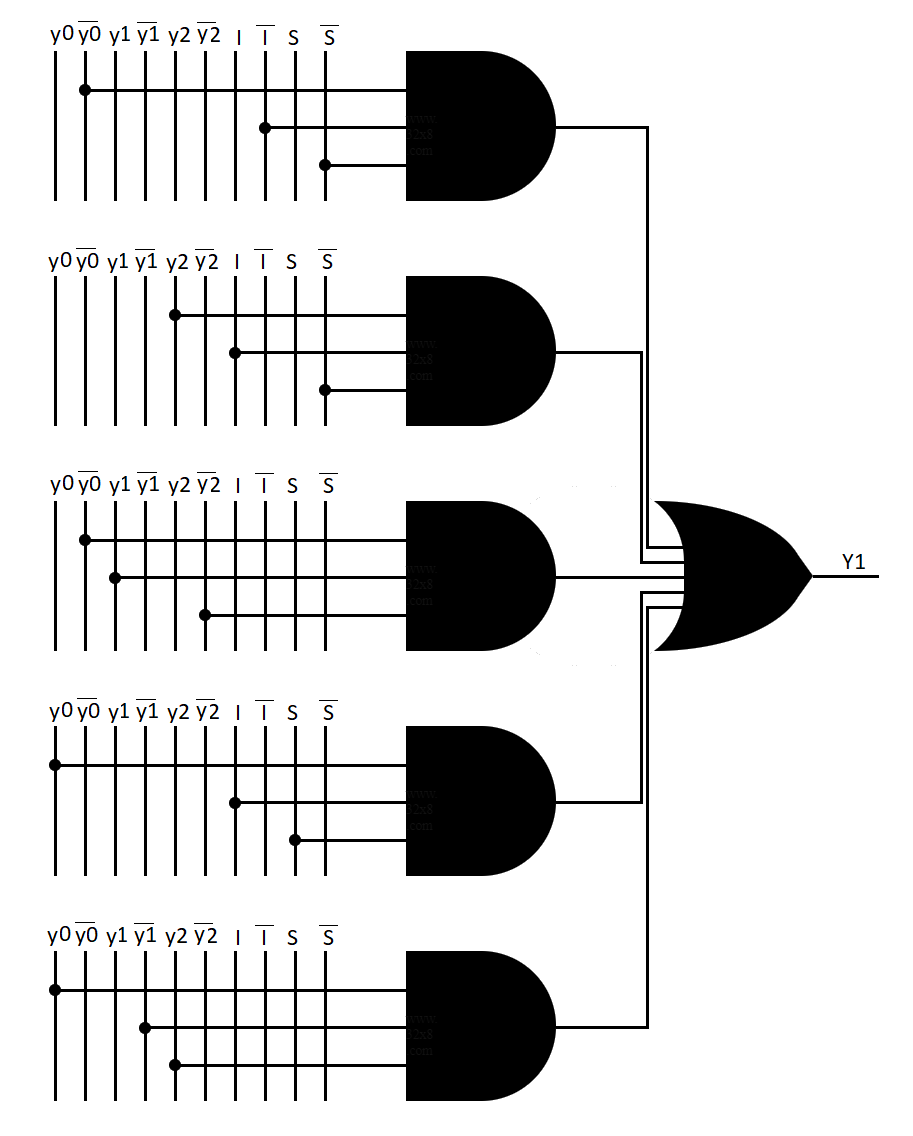
\includegraphics{figures/moore_Y1_schem.PNG}
	\caption{$Y_1$ schematic as a sum-of-products}
	\label{fig:ej1_moore_Y1_schem}
\end{figure}
\begin{figure}[H]
	\centering
	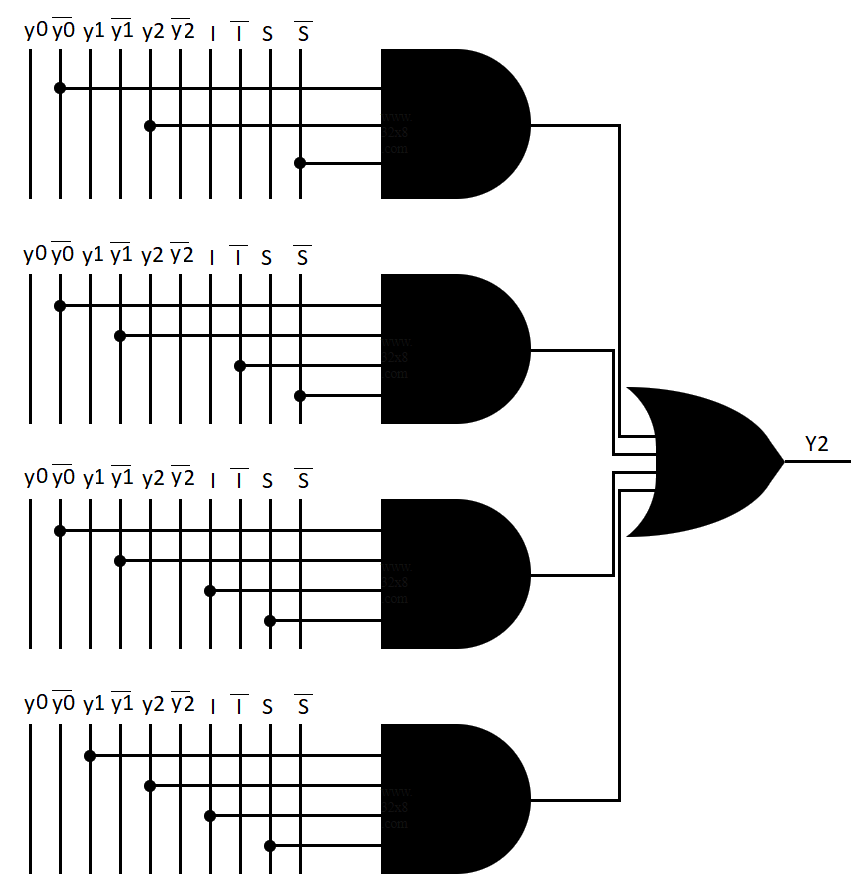
\includegraphics{figures/moore_Y2_schem.PNG}
	\caption{$Y_2$ schematic as a sum-of-products}
	\label{fig:ej1_moore_Y2_schem}
\end{figure}
\begin{figure}[H]
	\centering
	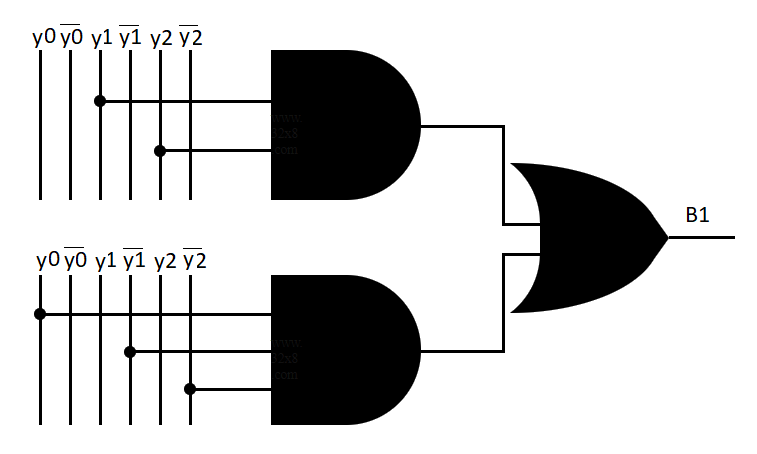
\includegraphics{figures/moore_B1_schem.PNG}
	\caption{$P_1$ schematic as a sum-of-products}
	\label{fig:ej1_moore_P1_schem}
\end{figure}
\begin{figure}[H]
	\centering
	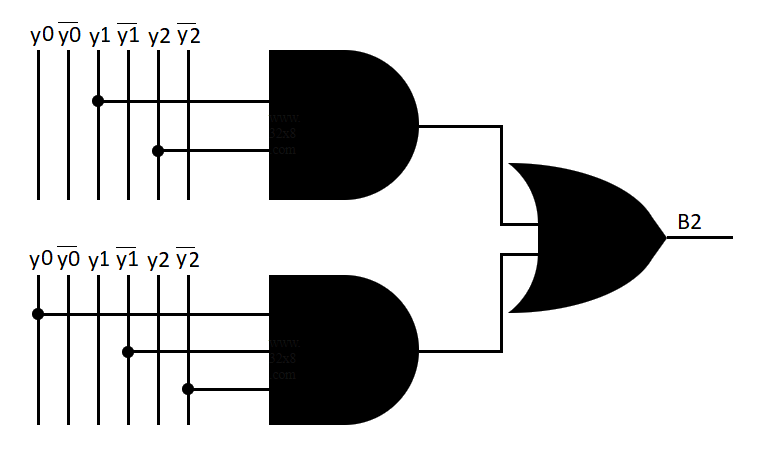
\includegraphics[scale=1]{figures/moore_B2_schem.PNG}
	\caption{$P_2$ schematic as a sum-of-products}
	\label{fig:ej1_moore_P2_schem}
\end{figure}



\section{Mealy-type FSM implementation}
\subsection{FSM flow-chart}
\begin{equation}
	\tikzfig{mealy_machine}
\end{equation}

The system can be implemented with a Mealy-type FSM with 4 states (see table \ref{tab:ej1_mealy_states}).

\subsection{State descriptions}
\begin{table}[H]	%mealy state descriptions
	\centering
	\begin{tabular}{|c|c|c|c|}
	\hline	
	$y_0, y_1$ & Name & Initials & Description\\	
	\hline 
	00 & Single pump: 1 &SP1& Pump 1 on\\ 
	\hline 
	01 & Next single pump: 2 &NSP2& Pump 1 and 2 both on or off. Next pump turned on alone: pump 2\\ 
	\hline 
	11 & Single pump: 2 &SP2& Only pump 2 is on\\ 
	\hline 
	10 & Next single pump: 1 &NSP1& Pump 1 and 2 both on or off. Next pump turned on alone: pump 1 \\ 
	\hline 
	\end{tabular} 
	\caption{Possible states for the Mealy-type FSM implementation.}
	\label{tab:ej1_mealy_states}
\end{table}

\subsection{State transition table}
\begin{table}[H]
	\centering
	\begin{tabular}{|c|c|c|c|c|}
		\hline 
		state\textbackslash I S & 00 & 01 & 11 & 10 \\ 
		\hline 
		SP1 & NSP2/11 & NSP1/00 & NSP2/00 & SP1/10 \\ 
		\hline 
		NSP2 & NSP2/11 & NSP1/00 & NSP2/00 & SP2/01 \\ 
		\hline 
		SP2 & NSP1/11 & NSP1/00 & NSP1/00 & SP2/01 \\ 
		\hline 
		NSP1 & NSP1/11 & NSP1/00 & NSP1/00 & SP1/10 \\ 
		\hline 
	\end{tabular} 
	\caption[States transitions and outputs for the Mealy-type FSM implementation]{States transitions and outputs for the Mealy-type FSM implementation. Each cell has the format $state\, initials \,/\, B_1\, B_2$}
	\label{tab:ej1_mealy_transitions}
\end{table}

The state transition and outputs are shown in table \ref{tab:ej1_mealy_transitions}. This can be separated in four other tables which correspond to the values of $Y_0$, $Y_1$, $B_1$, and $B_2$ for every combination of inputs and states ($I$, $S$, $y_0$ and $y_1$). Then, the minimal sum-of-products expressions for these variables are obtained. The result is shown below, while the procedure is presented in the appendix (section \ref{sec:ej1_appendix}). 

\subsection{Outputs and next states Karnaugh maps}
\begin{figure}[H]
	\centering
	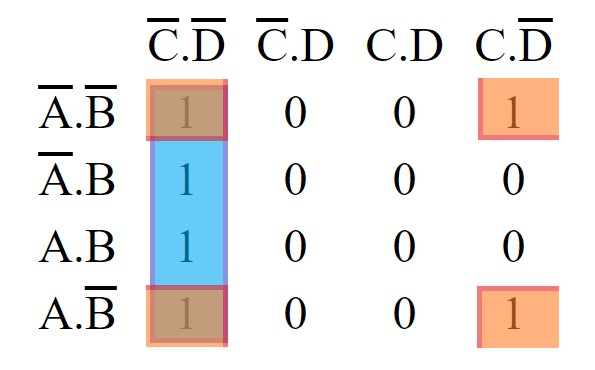
\includegraphics[scale=0.7]{figures/e3_tp3_ej1_mealy_b1_kmap.jpg}
	\caption{$P_1$ Karnaugh map}
\end{figure}
\begin{figure}[H]
	\centering
	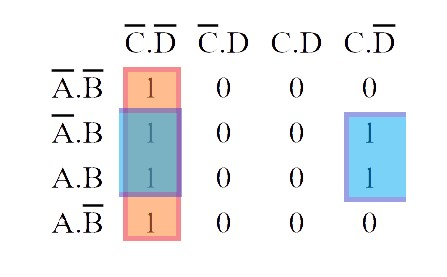
\includegraphics[scale=1]{figures/e3_tp3_ej1_mealy_b2_kmap.jpg}
	\caption{$P_2$ Karnaugh map}
\end{figure}
\begin{figure}[H]
	\centering
	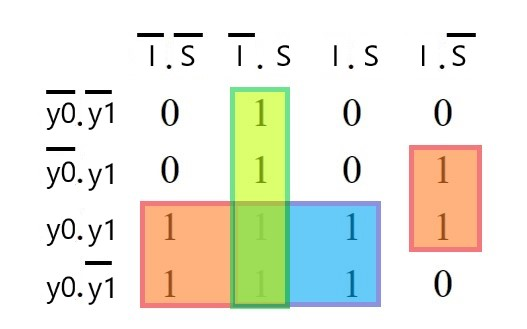
\includegraphics[scale=0.8]{figures/e3_tp3_ej1_mealy_y0_kmap.jpg}
	\caption{$y_0$ Karnaugh map}
\end{figure}
\begin{figure}[H]
	\centering
	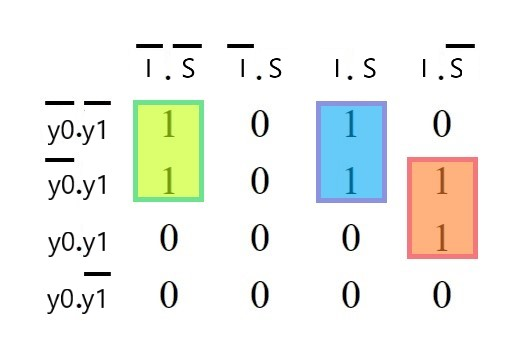
\includegraphics[scale=0.8]{figures/e3_tp3_ej1_mealy_y1_kmap.jpg}
	\caption{$y_1$ Karnaugh map}
\end{figure}



\subsection{Output and next states schematics}
%schematics as sum-of-products
\begin{figure}[H]
	\centering
	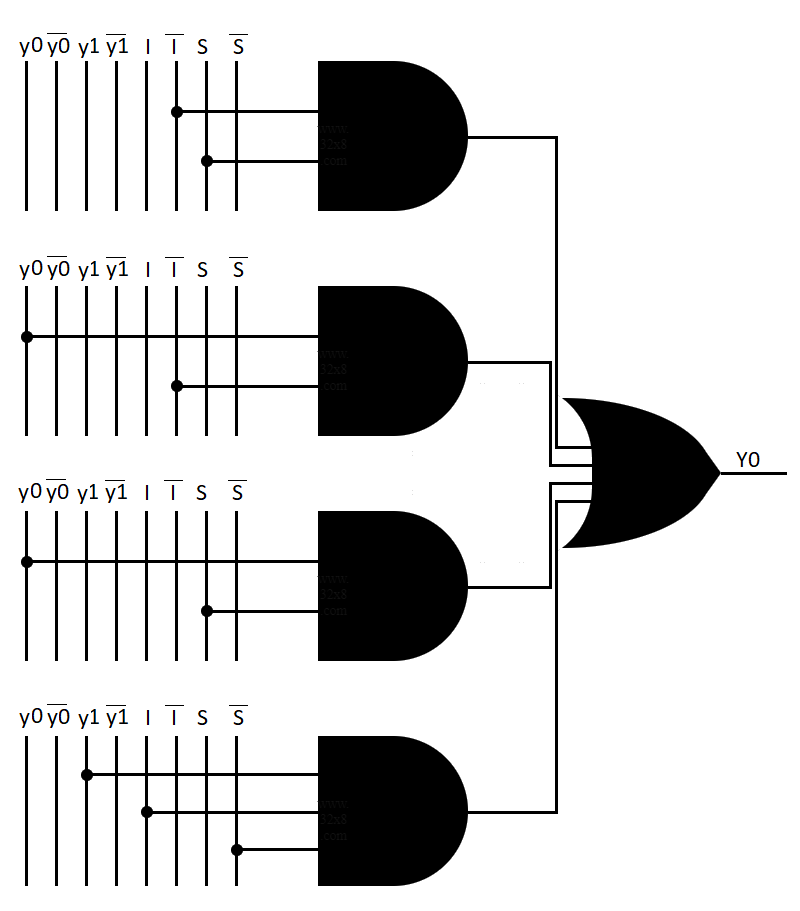
\includegraphics{figures/mealy_Y0_schem.PNG}
	\caption{$Y_0$ schematic as a sum-of-products}
	\label{fig:ej1_mealy_Y0_schem}
\end{figure}
\begin{figure}[H]
	\centering
	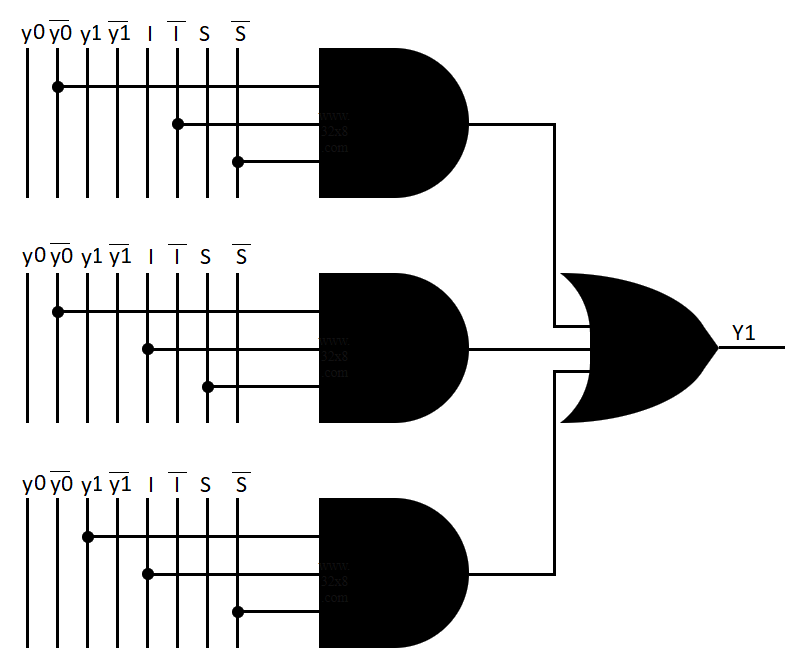
\includegraphics{figures/mealy_Y1_schem.PNG}
	\caption{$Y_1$ schematic as a sum-of-products}
	\label{fig:ej1_mealy_Y1_schem}
\end{figure}
\begin{figure}[H]
	\centering
	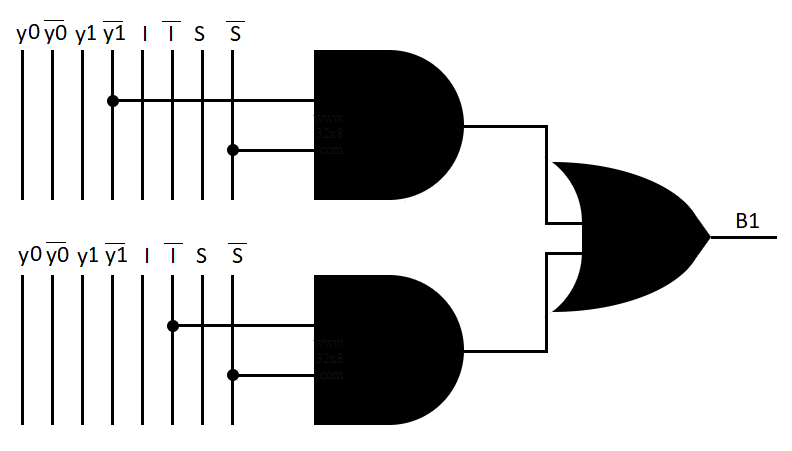
\includegraphics{figures/mealy_B1_schem.PNG}
	\caption{$P_1$ schematic as a sum-of-products}
	\label{fig:ej1_mealy_P1_schem}
\end{figure}
\begin{figure}[H]
	\centering
	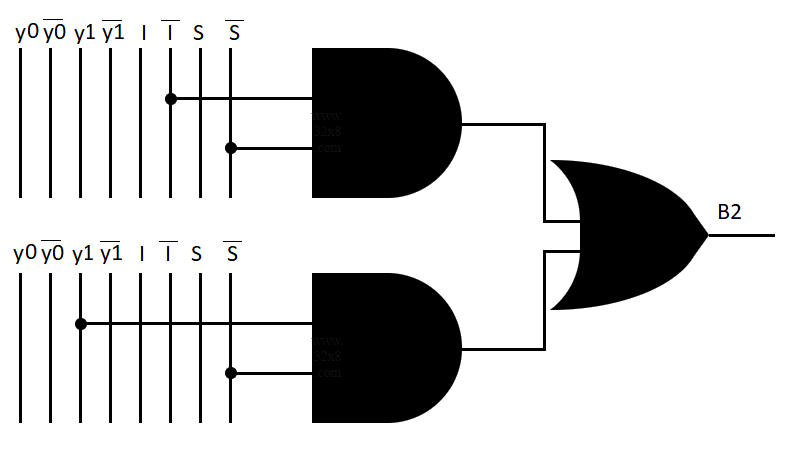
\includegraphics[scale=1]{figures/mealy_B2_schem.PNG}
	\caption{$P_2$ schematic as a sum-of-products}
	\label{fig:ej1_mealy_P2_schem}
\end{figure}


\end{document}
